\begin{figure}[h]
	\centering
	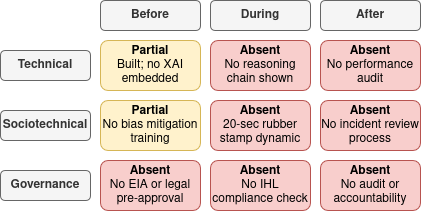
\includegraphics[width=0.8\textwidth]{images/analysis-chof.png}
	\caption{The CHOF framework for structuring ethical analysis across governance, socio-technical, and technical layers. Two yellow cells indicate where Habsora can be given partial compliance. The red cells indicate absence.}
	\label{fig:analysis-chof}
\end{figure}

\citet{info12090385}'s Comprehensive Human Oversight Framework (CHOF) was developed to assess accountability for autonomous systems whose internals are not directly inspectable. It divides oversight into a 3$\times$3 matrix, before, during and after deployment across a technical, socio-technical and governance mapping. The resulting matrix surfaces gaps which remain hidden when `human oversight` would be treated as a single requirement. Applying this framework to Habsora's implementation we get Figure~\ref{fig:analysis-chof}.

%The CHOF structures oversight across three layers: governance, socio-technical layer, and technical. Each of these layers is further analysed across three temporal phases: before, during, and after deployment of the autonomous weapon system. The governance layer concerns the legal and ethical conditions, investigating whether societal values and ethical principles are respected. The socio-technical layer focuses on the stakeholders involved, both the ones operating the system and those personally affected by it. The technical layer looks at the system itself, addressing issues such as automation bias and the system working as a black box, meaning the inner workings of the system are not transparent to users or stakeholders.


\subsection{Technical Layer}
Habsora has been described as an ensemble of deep learning models processing multimodal data \citep{abraham_2024, dwoskin_2024}. Such architectures are inherently opaque, \citet{arrieta2019explainableartificialintelligencexai} characterise this as the accuracy/interpretability trade-off, where deep ensembles maximize predictive performance at the cost of transparency. While post-hoc explainability methods exist that could be applied to such systems, reports on Habsora's use indicate that no such methods are applied as the operators point of decision.

This opacity directly links to the legal consequences. \citet{ootlaws} establish that IHL's distinction principle requires positive identification of a target as being a military objective. In conjunction with the proportionality assessment being understood by the user. Without any interpretability the legal review is effectively empty.

The above failures map directly into the highest-ranked principles identified by \citet{khan2021ethicsaisystematicliterature}. Both \textbf{P-01} transparency and \textbf{P-03} accountability, further compounded by their challenges: lack of technical understanding among decision-makers \textbf{CH-06} and the absence of binding legal frameworks \textbf{CH09}. While this might not be a failure of intent, it is a structural property of opaque architectures. Combined with lacking operator-facing interfaces, this creates a system which can not provide the context for understanding.


\subsection{Socio-technical}

The Value Sensitive Design (VSD) framework addresses indirect stakeholders, those affected without directly using the system, such as civilians in the target environment. Palestinian civilians were not involved in its design, and their values were not elicited to ground the system's targeting logic. They remain non-consenting parties who face the consequences of the system's use without recourse. There is a large asymmetry in consequences between those operating the system and those subjected to it.

% in VSD framework staat dat mensen die als stakeholder geraakt worden, ook betrokken moeten worden. 
% DEZE ZIN IS TOEGEVOEGD:
% \citet{friedman2008vsd}'s Value Sensitive Design framework adds to this by specifying indirect stakeholders, those affected without directly using the system, such as civilians in the target environment.



For IDF commanders, the conditions necessary for genuine human oversight are structurally not present. \citet{mhcof} argue that meaningful human control requires both sufficient information and meaningful freedom of action. Habsora undermines both: commanders receive recommendations without transparency into the underlying reasoning, and the short decision windows of the system leave almost no room for critical evaluation. \citet{miller2018explanationartificialintelligenceinsights} shows that from social science, without understanding what went into a decision, the explainee cannot meaningfully interrogate it. Combined with the large amount of targets the system generates, this reduces what would normally require extended deliberation and proportionality assessments to a button press. Former IDF commanders have described this process as `rubber-stamping'~\citep{kozlovski2024algorithms}. This confirms the presence of automation bias, which is when operators rely too much on AI outputs under time pressure~\citep{parasuraman2010complacency}.

The consequence is that IDF commanders formally bear moral and legal responsibility for strikes they cannot meaningfully evaluate, while the system's opacity diffuses accountability in practice. Targeting decisions that once demanded careful human judgement are now effectively delegated to an algorithm. This prevents the human control which the IHL demands, and that \citet{mhcof} identify as a precondition for attributing responsibility.

\subsection{Governance}

Article 36 of Protocol I to the Geneva Conventions requires countries to perform legal reviews of new weapons systems to determine whether their use would be prohibited under international law~\citep{icrc_api_article36_1977}. Israel is one of the few countries that have not ratified Protocol I~\citep{icrc_api_stateparties}. UNESCO maintains that delegating life-or-death decisions to an AI system is itself forbidden~\citep{aimag.v40i1.2848}. Yet, no accountability framework exists to enforce this in the case of Habsora \textbf{TODO EVIDENCE NEEDED}.
% Deze zin stond voor 'UNESCO maintains ...'
% This means it has no legal obligation to review Habsora's compliance with IHL prior to deployment. 

Once deployed, establishing accountability becomes difficult. Under IHL, commanders are legally responsible for how weapons are used, even when autonomous functions are involved~\citep{icrc_api_article86_1977}. They are judged on what they knew at the time of the decision~\citep{henckaerts2005customary}. In practice, responsibility is spread across developers, the algorithm, the receiving IDF officer, and the approving commander~\citep{aimag.v40i1.2848}. The Lavender system, the human-targetting extension of Habsora, has a documented 10\% error tolerance in targeting recommendations. XYZ  This illustrates the problem: this margin makes civilian casualties inevitable. In the midst of war, real-time monitoring is not easy to pull off, which compounds the issue.

% XYZ -> verwoord: als Lavender al zo'n hoge tolerance heeft, dan moet Habsora dat wellicht ook hebben
% 'human-targetting': Eventjes opzoeken hoe Habsora en Lavender samenwerken

After deployment, we find that review processes are largely absent. The system's opacity makes it difficult to determine whether casualties resulted from an AI recommendation or a human override. Palestinian civilians, who the most directly affected stakeholders, were never consulted. No structured ethical assessment, such as `value sensitive design' (VSD), was conducted.


% Eerste zin herschrijven:
    % UNESCO regeling, veel mensen hebben het getekend
    % Er is duidelijk een oversight mechanism
    % Maar we hebben er niks over kunnen vinden ivm Israel, nochtans zou dit publieke info moeten zijn


% Eerst kort VSD uitleggen, bruggetje maken van '?

